Our setting consists of three qubits: the Drive, System and Transducer qubit. The Drive and Transducer qubits can be set by the experimenter in N discrete steps modelled as piecewise constant functions of ($\theta_D, \phi_D$) and ($\theta_T, \phi_T$) respectively (see figure \ref{pwc}), the system qubit is initialised in a pure state.
In general, unitary evolution of a multipartite system will lead to entanglement, meaning Drive and Transducer bits are no longer pure states. This is at odds with the assumption of piecewise constant control functions. We therefore model Drive and Transducer qubits as series of ancilla qubits which interact with the system such that the state does not entangle and can afterwards be measured \cite{beyer2020}.
In the remainder of this work we use the interaction Hamiltonian on the three qubit Hilbert space
\begin{equation*}
	H_{DST} = H_{I} \otimes \mathbb{1} + \mathbb{1} \otimes H_{I}, \\
	H_{I} = \sigma_{+} \otimes \sigma_{-} + \sigma_{-} \otimes \sigma_{+}
\end{equation*}
unless otherwise noted.
The time evolution and work extraction is then calculated as follows, where $\Delta t$ is time span between qubit switching:
\begin{align}
	H_S^i = \bra{\psi_D^i}\bra{\psi_T^i} H_{DST} \ket{\psi_D^i} \ket{\psi_T^i} \\
	\rho_S^{i+1} = U^i \rho_S^i U^{i\dagger}, \ U^i = e^{-iH_S^i \Delta t} \\
	W = - \Sigma_i \mathrm{Tr} \ \rho_S^i \ dH_S^i \\
	dH_S^i = \bra{\psi_D^i}\bra{\psi_T^{i+1}} H_{DST} \ket{\psi_D^i} \ket{\psi_T^{i+1}} - \bra{\psi_D^i}\bra{\psi_T^i} H_{DST} \ket{\psi_D^i} \ket{\psi_T^i}.	
\end{align}
Here we use the partial Hamiltonian $H_S^i$ on S at time step $i \in [1, N - 1]$, as well as corresponding system density matrix $\rho_S^i$.

\begin{figure}
	\centering
	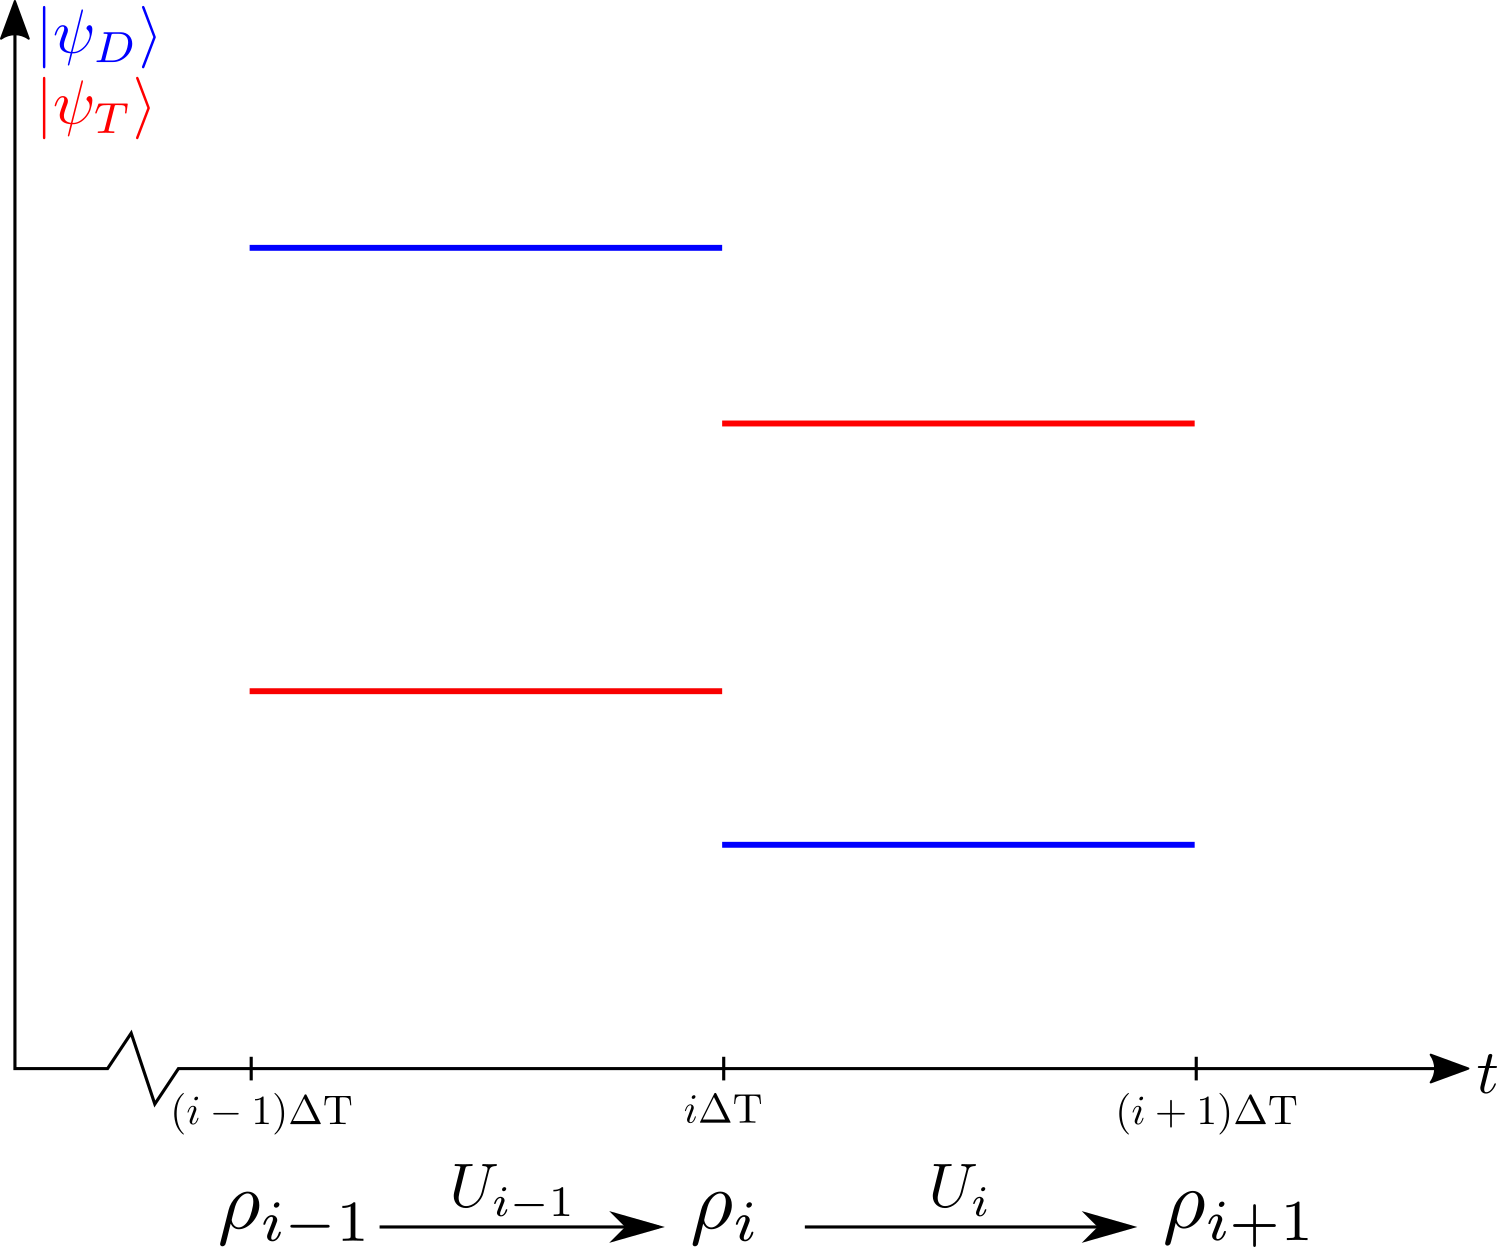
\includegraphics[width=0.6\textwidth]{img/pwc}
	\caption{Piecewise constant implementation of Drive and Transducer qubits. The vertical axis shows qubit state in arbitrary units. The qubit states are switched instantaneously and then kept constant for $\Delta t$ while $\rho_S$ evolves unitarily.}
	\label{pwc}
\end{figure}